%%%%%%%%%%%%%%%%%%%%%%%%%%%%%%%%%
%%% DOCUMENT GENERAL SETTINGS %%%
%%%%%%%%%%%%%%%%%%%%%%%%%%%%%%%%%
\documentclass[a4paper,11pt]{book}

%%%%%%%%%%%%%%%%%%%%%%%%%%%%%%%%%
%%%%%%%%%%% PREAMBLE %%%%%%%%%%%%
%%%%%%%%%%%%%%%%%%%%%%%%%%%%%%%%%

% ********************************************************************
% Packages
% ********************************************************************
% Useful to add source code blocks of any programming language.
% Package wiki: https://en.wikibooks.org/wiki/LaTeX/Source_Code_Listings
\usepackage{listings}

% Useful to add non-english special characters.
% Package wiki: https://en.wikibooks.org/wiki/LaTeX/Internationalization
\usepackage[utf8]{inputenc}

% Load Spanish language settings using '.' as decimal separator.
% Package wiki: https://en.wikibooks.org/wiki/LaTeX/Internationalization#Babel
% Package wiki: https://en.wikibooks.org/wiki/LaTeX/Internationalization#Spanish
\usepackage[spanish]{babel}

% \usepackage[style=list, number=none]{glossary} %
%\usepackage{titlesec}
%\usepackage{pailatino}

\decimalpoint

% Useful to align number columns.
% Package wiki: https://en.wikibooks.org/wiki/LaTeX/Tables#Aligning_columns_at_decimal_points_using_dcolumn
\usepackage{dcolumn}

\newcolumntype{.}{D{.}{\esperiod}{-1}}
\makeatletter % changes the catcode of @ to 11: Explanation -> https://tex.stackexchange.com/questions/8351/what-do-makeatletter-and-makeatother-do
\addto\shorthandsspanish{\let\esperiod\es@period@code}
\makeatother % changes the catcode of @ back to 12


% Useful to add algorithms.
% Package wiki: https://en.wikibooks.org/wiki/LaTeX/Algorithms
\usepackage[chapter]{algorithm}

% Require verbatim enviroment. It allows us to make blocks which wont be interpreted by the compiler.
% Package wiki: https://en.wikibooks.org/wiki/LaTeX/Paragraph_Formatting#Verbatim_text
\RequirePackage{verbatim}
%\RequirePackage[Glenn]{fncychap}

% Useful to make customize header and footers.
% Package wiki: https://en.wikibooks.org/wiki/LaTeX/Customizing_Page_Headers_and_Footers#Customizing_with_fancyhdr
\usepackage{fancyhdr}

% Useful to import graphic content.
% Package wiki: https://en.wikibooks.org/wiki/LaTeX/Importing_Graphics
\usepackage{graphicx}

% Useful to execute commands after the next page break.
% Package info: https://www.ctan.org/pkg/afterpage
\usepackage{afterpage}

% Useful to add tables functionality
% Package wiki: https://en.wikibooks.org/wiki/LaTeX/Tables
\usepackage{longtable}

% Useful to add colors to table rows and columns.
% Package info: https://www.ctan.org/pkg/colortbl
\usepackage{colortbl}

% Useful to add hyperlinks or urls.
% Package wiki: https://en.wikibooks.org/wiki/LaTeX/Hyperlinks
\usepackage[pdfborder={000}]{hyperref} %referencia

% Useful to add urls with description.
% Package info: https://www.stack.nl/~jwk/latex/examples/node4.html
\usepackage{url}

% Allow us to change the typesetting of footnotes.
% Package info: https://www.ctan.org/pkg/footmisc
\usepackage[stable]{footmisc}

% Allow us to add a document index.
% Package info: https://en.wikibooks.org/wiki/LaTeX/Indexing
\usepackage{makeidx}

% Allow us to add a document glossary.
% Package info: https://en.wikibooks.org/wiki/LaTeX/Glossary
\usepackage{glossaries}

% Deal with end of line issues.
% Package info: https://www.ctan.org/pkg/xspace
\usepackage{xspace}

% Allow us to use multiple columns
\usepackage{multicol}

% ********************************************************************
% Re-usable information
% ********************************************************************
\newcommand{\myTitle}{Reconocimiento de Expresiones Faciales\xspace}
\newcommand{\mySubtitle}{por Computador\xspace}
\newcommand{\myKeywords}{Reconocimiento, expresión, facial, visión, computador, aprendizaje, automático, redes, neuronales, convolucionales.\xspace}
\newcommand{\myDegree}{Grado en Ingeniería Informática\xspace}
\newcommand{\myName}{Francisco José Fajardo Toril\xspace}
\newcommand{\myDNI}{76424577Q\xspace}
\newcommand{\myProf}{Miguel García Silvente\xspace}
\newcommand{\myOtherProf}{Eugenio Aguirre Molina\xspace}
%\newcommand{\mySupervisor}{Put name here\xspace}
\newcommand{\myFaculty}{Escuela Técnica Superior de Ingenierías Informática y de
	Telecomunicación\xspace}
\newcommand{\myFacultyShort}{E.T.S. de Ingenierías Informática y de
	Telecomunicación\xspace}
\newcommand{\myDepartment}{Ciencias de la Computación e Inteligencia Artificial\xspace}
\newcommand{\myUni}{\protect{Universidad de Granada}\xspace}
\newcommand{\myLocation}{Granada\xspace}
\newcommand{\myTime}{\today\xspace}
\newcommand{\myVersion}{Version 0.1\xspace}

% English info.
\newcommand{\myTitleEN}{Facial Expression Recognition\xspace}
\newcommand{\mySubtitleEN}{by Computer\xspace}
\newcommand{\myKeywordsEN}{Facial, expression, recognition, computer, vision, machine, learning, convolutional, neural, network.\xspace}


% "hyperref" package options
\hypersetup{
	pdfauthor = {\myName (frannn@correo.ugr.es)},
	pdftitle = {\myTitle},
	pdfsubject = {},
	pdfkeywords = {\myKeywords},
	pdfcreator = {LaTeX con el paquete ....},
	pdfproducer = {pdflatex}
}

%\hyphenation{}

% ********************************************************************
% Packages configuration.
% ********************************************************************

%\usepackage{doxygen/doxygen}
%\usepackage{pdfpages}


%\usepackage{index}

\makeindex
%\usepackage[style=long, cols=2,border=plain,toc=true,number=none]{glossary}
\makeglossary

% Definición de comandos que me son tiles:
\renewcommand{\indexname}{Índice alfabético}
\renewcommand{\glossaryname}{Glosario}

\pagestyle{fancy}
\fancyhf{}
\fancyhead[LO]{\leftmark}
\fancyhead[RE]{\rightmark}
\fancyhead[RO,LE]{\textbf{\thepage}}
\renewcommand{\chaptermark}[1]{\markboth{\textbf{#1}}{}}
\renewcommand{\sectionmark}[1]{\markright{\textbf{\thesection. #1}}}

\setlength{\headheight}{1.5\headheight}

\newcommand{\HRule}{\rule{\linewidth}{0.5mm}}
%Definimos los tipos teorema, ejemplo y definición podremos usar estos tipos
%simplemente poniendo \begin{teorema} \end{teorema} ...
\newtheorem{teorema}{Teorema}[chapter]
\newtheorem{ejemplo}{Ejemplo}[chapter]
\newtheorem{definicion}{Definición}[chapter]

\definecolor{gray97}{gray}{.97}
\definecolor{gray75}{gray}{.75}
\definecolor{gray45}{gray}{.45}
\definecolor{gray30}{gray}{.94}

\lstset{ frame=Ltb,
     framerule=0.5pt,
     aboveskip=0.5cm,
     framextopmargin=3pt,
     framexbottommargin=3pt,
     framexleftmargin=0.1cm,
     framesep=0pt,
     rulesep=.4pt,
     backgroundcolor=\color{gray97},
     rulesepcolor=\color{black},
     %
     stringstyle=\ttfamily,
     showstringspaces = false,
     basicstyle=\scriptsize\ttfamily,
     commentstyle=\color{gray45},
     keywordstyle=\bfseries,
     %
     numbers=left,
     numbersep=6pt,
     numberstyle=\tiny,
     numberfirstline = false,
     breaklines=true,
   }

% minimizar fragmentado de listados
\lstnewenvironment{listing}[1][]
   {\lstset{#1}\pagebreak[0]}{\pagebreak[0]}

\lstdefinestyle{CodigoC}
   {
	basicstyle=\scriptsize,
	frame=single,
	language=C,
	numbers=left
   }
\lstdefinestyle{CodigoC++}
   {
	basicstyle=\small,
	frame=single,
	backgroundcolor=\color{gray30},
	language=C++,
	numbers=left
   }


\lstdefinestyle{Consola}
   {basicstyle=\scriptsize\bf\ttfamily,
    backgroundcolor=\color{gray30},
    frame=single,
    numbers=none
   }


\newcommand{\bigrule}{\titlerule[0.5mm]}


%Para conseguir que en las páginas en blanco no ponga cabecerass
\makeatletter
\def\clearpage{%
  \ifvmode
    \ifnum \@dbltopnum =\m@ne
      \ifdim \pagetotal <\topskip
        \hbox{}
      \fi
    \fi
  \fi
  \newpage
  \thispagestyle{empty}
  \write\m@ne{}
  \vbox{}
  \penalty -\@Mi
}
\makeatother

\usepackage{pdfpages}

%%%%%%%%%%%%%%%%%%%%%%%%%%%%%%%%%
%%%%%%%%%%% DOCUMENT %%%%%%%%%%%%
%%%%%%%%%%%%%%%%%%%%%%%%%%%%%%%%%

\begin{document}
\begin{titlepage}
 
 
\newlength{\centeroffset}
\setlength{\centeroffset}{-0.5\oddsidemargin}
\addtolength{\centeroffset}{0.5\evensidemargin}
\thispagestyle{empty}

\noindent\hspace*{\centeroffset}\begin{minipage}{\textwidth}

\centering

\includegraphics[width=0.9\textwidth]{imagenes/logo_ugr.jpg}\\[1.4cm]

\textsc{ \Large TRABAJO FIN DE GRADO\\[0.2cm]}
\textsc{ INGENIERÍA EN INFORMÁTICA }\\[1cm]
% Upper part of the page
% 
% Title
{\Huge\bfseries \myTitle\\
}
\noindent\rule[-1ex]{\textwidth}{3pt}\\[3.5ex]
\end{minipage}

\vspace{2.0cm}
\noindent\hspace*{\centeroffset}\begin{minipage}{\textwidth}
\centering

\textbf{Autor}\\ {\myName}\\[2.5ex]
\textbf{Directores}\\
{\myProf\\
\myOtherProf}\\[2cm]

\includegraphics[width=0.3\textwidth]{imagenes/etsiit_logo.png}\\[0.1cm]
\textsc{\myFaculty}\\
\textsc{---}\\
\myLocation, \myTime 
\end{minipage}
%\addtolength{\textwidth}{\centeroffset}
%\vspace{\stretch{2}}
\end{titlepage}



\chapter*{}
%\thispagestyle{empty}
%\cleardoublepage

%\thispagestyle{empty}

\begin{titlepage}
 
 
\setlength{\centeroffset}{-0.5\oddsidemargin}
\addtolength{\centeroffset}{0.5\evensidemargin}
\thispagestyle{empty}

\noindent\hspace*{\centeroffset}\begin{minipage}{\textwidth}

\centering
%
\includegraphics[width=0.9\textwidth]{imagenes/logo_ugr.jpg}\\[1.4cm]

%\textsc{ \Large PROYECTO FIN DE CARRERA\\[0.2cm]}
%\textsc{ INGENIERÍA EN INFORMÁTICA}\\[1cm]
% Upper part of the page
% 

 \vspace{3.3cm}

%si el proyecto tiene logo poner aquí

\includegraphics{imagenes/logo.png} 
 \vspace{0.5cm}

% Title

{\Huge\bfseries \myTitle\\
}
\noindent\rule[-1ex]{\textwidth}{3pt}\\[3.5ex]
{\large\bfseries \mySubtitle.\\[4cm]}
\end{minipage}

\vspace{2.5cm}
\noindent\hspace*{\centeroffset}\begin{minipage}{\textwidth}
\centering

\textbf{Autor}\\ {\myName}\\[2.5ex]
\textbf{Directores}\\
{\myProf\\
\myOtherProf}\\[2cm]
%
\includegraphics[width=0.15\textwidth]{imagenes/tstc.png}\\[0.1cm]
%\textsc{Departamento de Teoría de la Señal, Telemática y Comunicaciones}\\
%\textsc{---}\\
%Granada, mes de 201
\end{minipage}
%\addtolength{\textwidth}{\centeroffset}
\vspace{\stretch{2}}

 
\end{titlepage}






\cleardoublepage
\thispagestyle{empty}

\begin{center}
{\large\bfseries \myTitle}\\
\end{center}
\begin{center}
\myName\\
\end{center}

%\vspace{0.7cm}
\noindent{\textbf{Palabras clave}: \myKeywords}\\

\vspace{0.7cm}
\noindent{\textbf{Resumen}}\\

El objetivo de este documento es mostrar al lector el proceso seguido para el desarrollo de una aplicación software capaz de resolver el problema del reconocimiento de expresiones faciales por computador. Esto es, asignar a una imagen la etiqueta que mejor describe la expresión facial que esa imagen representa. Para la resolución de este problema se entrenará un clasificador basado en redes neuronales convolucionales, que etiquetará la imagen de entrada proporcionada por el usuario mediante una interfaz simple e intuitiva.

\cleardoublepage


\thispagestyle{empty}


\begin{center}
{\large\bfseries \myTitleEN}\\
\end{center}
\begin{center}
\myName\\
\end{center}

%\vspace{0.7cm}
\noindent{\textbf{Keywords}: \myKeywordsEN}\\

\vspace{0.7cm}
\noindent{\textbf{Abstract}}\\

This document main objective is to show the reader the process I followed to develop a software application which is able to solve the face expression recognition problem through computer. This implies to assign to an image, the tag that better describes the facial expression that is represented in that image. To solve this problem, I will train a convolutional neural network based model that will classify the image chosen by the final user through a simple and intuitive user interface.

\chapter*{}
\thispagestyle{empty}

\noindent\rule[-1ex]{\textwidth}{2pt}\\[4.5ex]

Yo, \textbf{\myName}, alumno de la titulación \myDegree de la \textbf{\myFaculty de la \myUni}, con DNI \myDNI, autorizo la
ubicación de la siguiente copia de mi Trabajo Fin de Grado en la biblioteca del centro para que pueda ser
consultada por las personas que lo deseen.

\vspace{6cm}

\noindent Fdo: \myName

\vspace{2cm}

\begin{flushright}
\myLocation a \myTime .
\end{flushright}


\chapter*{}
\thispagestyle{empty}

\noindent\rule[-1ex]{\textwidth}{2pt}\\[4.5ex]

D. \textbf{\myProf}, Profesor del Área de \myDepartment del Departamento de Ciencias de la Computación e I.A. de la \myUni.

\vspace{0.5cm}

D. \textbf{\myOtherProf}, Profesor del Área de \myDepartment del Departamento de Ciencias de la Computación e I.A. de la \myUni.


\vspace{0.5cm}

\textbf{Informan:}

\vspace{0.5cm}

Que el presente trabajo, titulado \textit{\textbf{\myTitle}},
ha sido realizado bajo su supervisión por \textbf{\myName}, y autorizamos la defensa de dicho trabajo ante el tribunal
que corresponda.

\vspace{0.5cm}

Y para que conste, expiden y firman el presente informe en Granada a \myTime.

\vspace{1cm}

\textbf{Los directores:}

\vspace{5cm}

\noindent \textbf{\myProf \ \ \ \ \ \myOtherProf}

\chapter*{Agradecimientos}
\thispagestyle{empty}
\vspace{1cm}
En primer lugar agradecer a mis tutores \textbf{\myProf} y \textbf{\myOtherProf} por resolver mis dudas y aportar ideas y ofrecer su punto de vista durante el desarrollo de este trabajo.\\

En segundo lugar agradecer a todas las personas implicadas en el desarrollo y mantenimiento de las herramientas open source que he usado (Apartado \ref{sub:software}) tales como: \textit{OpenCV}\cite{opencv}, \textit{Dlib}\cite{dlib} y \textit{Caffe}\cite{caffe}, así como otras que he empleado para el desarrollo de este documento como son: \textit{TeXstudio}\cite{texstudio} y \textit{yEd}\cite{yed}. \\

Por último agradecer a todas las personas involucradas en la producción de la base de datos empleada en este trabajo: Yalefaces\cite{yalefaces} y Karolinska Directed Emotional Faces\cite{kdef98} (KDEF).


%\frontmatter
%\tableofcontents
%\listoffigures
%\listoftables

%
%\mainmatter
%\setlength{\parskip}{5pt}

%\input{capitulos/01_Introduccion}

\chapter{Introducción}

%\ Aquí hay que contextualizar el TFG, es decir, explicar la motivación que existe para realizar el TFG describiendo la realidad de la que se parte haciendo un estudio del estado del arte breve con referencias bibliográficas a trabajos que han tratado también el tema que vamos a abordar.

\section{Motivación}

El problema del reconocimiento de expresiones faciales es un paso adelante tras resolver el problema del reconocimiento facial en imágenes. Tal y como mencioné en el resumen puede ser descrito de la siguiente manera:
\begin{center}
	\textit{Dada una imagen de entrada, obtener la etiqueta de salida que mejor identifique la expresión facial que aparece en dicha imagen.}\\
\end{center}

A priori la solución para un ser humano es trivial. Tenemos muchas maneras de adivinar el estado de ánimo de una persona, pero si tenemos que basarnos en nuestra visión, una posible solución sería:
\textit{"Simplemente observa los rasgos faciales del sujeto e intenta adivinar su estado de ánimo basándote en tu experiencia pasada con otros seres humanos."\\}

Imagine que deseamos desarrollar un agente basado en inteligencia artificial para que interactúe con otros seres humanos. Sería de gran utilidad que este agente basara sus acciones en función del estado de ánimo de la persona/as con las que está comunicándose para lograr de esta forma un mayor grado de comprensión o empatía. De la misma manera podríamos pensar en una aplicación que escoge la música idónea para nosotros en función de nuestro estado de ánimo en ese momento a través de una captura mediante la cámara del computador.

\subsection{Trabajos relacionados}

Como se puede ver, la solución a este problema puede ser de utilidad en diversas aplicaciones del mundo real, sin embargo, ¿Cómo podría un computador resolver este problema? Hay diversas propuestas que han tratado de resolver este problema.

\subsubsection{Facial Expression Analysis using Active Shape Model\cite{shbib_zhou15}}

Active Shape Model(ASM)\cite{cootes_taylor_cooper_graham94} es una técnica que permite, dada una imagen del objeto para el que fue entrenado, localizar un conjunto de puntos de referencia previamente definidos tal y como se puede ver en la Figura \ref{fig:landmarks}. En el caso de un rostro humano estos puntos pueden estar los principales indicadores de la expresión facial, como pueden ser las cejas, boca, ojos...\\
En este paper \cite{shbib_zhou15} en concreto, se tienen en cuenta para cada cara, 68 puntos de referencia. Se procesan los puntos extraídos y se obtiene un modelo geométrico para ese rostro concreto. Acto seguido, haciendo uso de la técnica de clasificación conocida como Support Vector Machine(SVM), se clasifica ese modelo geométrico para predecir a qué expresión facial pertenece obteniendo un porcentaje de acierto del 92,1\%.

\begin{figure}[!]
\centering
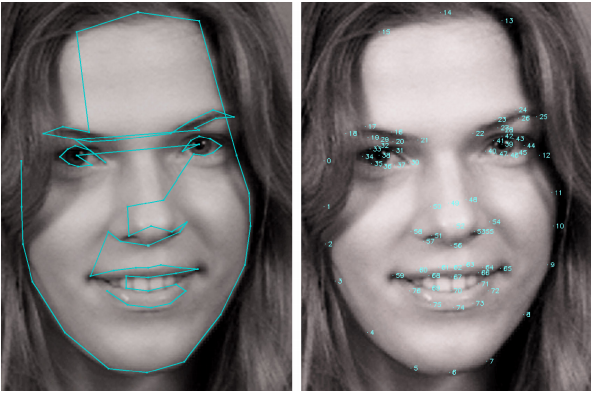
\includegraphics[width=0.7\linewidth]{imagenes/landmarks}
\caption[Puntos de Referencia ASM]{Puntos de Referencia extraídos con ASM.}
\label{fig:landmarks}
\end{figure}


\subsubsection{Facial expression recognition and synthesis based on an appearance model\cite{abboud_davoine_dang04}}
En este caso se hace uso de la técnica \textit{Active Appearance Model (AAM)}\cite{cootes_edwards_taylor98}, un método estadístico que se emplea para emparejar, un modelo geométrico, a una nueva forma del mismo tipo para el que fue entrenado, pero que el modelo no ha visto antes, como por ejemplo un nuevo rostro humano. Esta técnica (AAM)  es una generalización de la ya antes mencionada ASM\cite{cootes_taylor_cooper_graham94}.
Además, lo que en este caso se intenta es que la información usada esté exenta de redundancia por lo que se aplican técnicas de aprendizaje no supervisado en una fase de preprocesamiento de la información como \textit{Análisis de Componentes Principales (PCA)} o \textit{Análisis de Componentes Independientes(ICA)} para reducir la dimensionalidad de la información  en una fase de preprocesamiento. En este caso obtienen alrededor de un 84\% de acierto.

% Una vez descrito el marco general, se explica lo que se quiere hacer con el proyecto con la propuesta concreta que se pretende conseguir.
\subsection{¿Qué se pretende conseguir con este proyecto?}
\label{subsec:aspirations}
\begin{figure}[!]
	\centering
	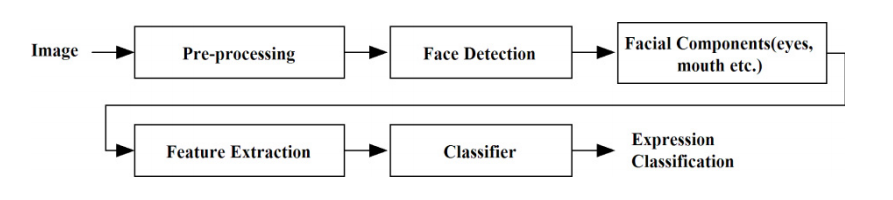
\includegraphics[width=0.7\linewidth]{imagenes/feg_diagram}
	\caption[Diagrama FER]{Diagrama general del proceso de reconocimiento.}
	\label{fig:feg_diagram}
\end{figure}
Las técnicas de ASM\cite{cootes_taylor_cooper_graham94} y AAM\cite{cootes_edwards_taylor98} son sensibles a rotaciones de la imagen, es decir, será difícil extraer los puntos de referencia en imágenes que disten mucho del concepto de imagen frontal, como por ejemplo una la fotografía de una persona mirando hacia un lado con una expresión facial determinada. Además, en la Figura \ref{fig:feg_diagram} extraída del siguiente paper\cite{kumari_rajesh_pooja15}, se puede ver el proceso general que se sigue a la hora de clasificar una imagen, en nuestro caso reconocimiento de expresiones faciales.\\

\begin{figure}[h!]
	\centering
	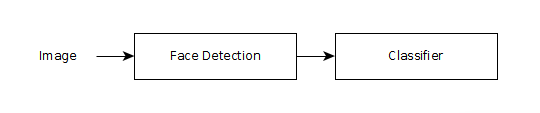
\includegraphics[width=0.7\linewidth]{imagenes/my_fer_diagram}
	\caption[my_diagram]{Diagrama del proceso objetivo.}
	\label{fig:my_fer_diagram}
\end{figure}

La idea principal que se quiere conseguir para resolver el problema consiste en simplificar de alguna manera dicho diagrama para que se asemeje al de la Figura \ref{fig:my_fer_diagram} de forma que no sea necesario extraer características cada vez que se clasifique una nueva imagen. Otra de las propuestas es que la rotación de la imagen de entrada no suponga un handicap a la hora de clasificarla. El propósito de estas medidas es:\\
\begin{itemize}
	\item Ganar en robustez con imágenes rotadas o inclinadas.
	\item Realizar la clasificación en tiempo real simplificando el preprocesamiento de las imágenes.
	\item Combinar todo en una aplicación de escritorio con una interfaz simple por encima para que cualquier usuario pueda utilizarla.
\end{itemize}

% Se termina explicando la organización de la memoria diciendo lo que se trata en cada capítulo.
\subsection{Organización del documento}
Este documento tratará de explicar el proceso seguido para el desarrollo de este trabajo. Para ello, se estructurará en los siguientes capítulos:\\
\begin{description}
	\item [Portada] - Información básica sobre el nombre del proyecto, la institución, el autor y los tutores.
	\item [Prefacio] - Resumen, palabras clave y agradecimientos.
	\item [Introducción] - Motivación del trabajo y estado del arte de este campo de investigación.  
	\item [Objetivos] - Se planteará un objetivo principal el cual será dividido en sub-objetivos más simples para poder llevar a cabo la tarea principal así como un resumen de las técnicas aprendidas durante la formación académica empleadas en este trabajo.
	\item [Resolución del trabajo] - Este capítulo se dividirá en varias secciones, en las que se explicará el método de ingeniería del software empleado para la resolución del trabajo, así como los recursos hardware y software, la especificación de requisitos, planificación, análisis funcional e implementación de la aplicación.
	\item [Conclusión] - Se hará una valoración del producto final y se valorará si se han alcanzaron o no los objetivos iniciales y en qué medida, teniendo en cuenta los puntos fuertes y débiles de la solución.
	\item [Bibliografía] - Referencias y citas bibliográficas usadas.
	\item [Anexo] - Pequeño manual de cómo usar la aplicación.
\end{description} 

\chapter{Objetivos}
\section{Objetivo principal}
%Objetivo general a conseguir: se enuncia lo que se quiere hacer sin entrar en detalles.
\begin{center}
	\textit{Desarrollar una aplicación de escritorio que dada una imagen detecte si aparece un rostro humano y en que en caso afirmativo, sea capaz de mostrar por pantalla, la etiqueta que mejor identifica la expresión facial que presenta dicho rostro.}\\
\end{center}
Se ha de cumplir este objetivo sin olvidar qué es lo que se pretende alcanzar con este trabajo (\ref{subsec:aspirations}). Esto es, simplificar el proceso de pre-procesamiento de las imágenes y de esta forma ver si es factible un proceso de clasificación en tiempo real. Teniendo esto en mente, dividiremos el objetivo principal en distintas fases o sub-tareas.

\section{Objetivos específicos}
% Objetivos específicos: Es dividir el objetivo general en los pasos a seguir con sub-objetivos más simples.
% Dicho de otro modo, son cada uno de los pasos a realizar para alcanzar el objetivo general, es decir solucionando todos y cada uno de los objetivos específicos se resuelve el objetivo general. (Poner entre 3 y 5 como mucho).
%%%%%%%%%%%%%%%%%%%% Se puede decir en qué apartado se tratará cada objetivo específico. %%%%%%%%%%%%%%%%%%%%%%
\begin{enumerate}
	\item Preparación de la información con la que entrenaremos el clasificador.
	\begin{enumerate}
		\item Obtener una base de datos.
		\item Pre-procesamiento de la información.
		\item Creación del conjunto de training, validación y test.
	\end{enumerate}
	\item Entrenamiento del clasificador.
	\begin{enumerate}
		\item Selección de parámetros.
		\item Realización de pruebas (Vuelta al paso 2 si es necesario).
	\end{enumerate}
	\item Desarrollo de interfaz que haga uso del clasificador.
\end{enumerate}

%Poner también los aspectos formativos previos utilizados, por ejemplo si se han usado técnicas de visión concretas como Transformada de Hough, Método de detección de rostros Viola-Jones, Filtro de Partículas, o técnicas de aprendizaje por SVM, etc. Se explica un poco cada método.
\section{Técnicas empleadas}
Hasta ahora hemos hablado de objetivos, sin entrar demasiado en detalle acerca de qué técnicas serán las que emplearemos para llevarlos a cabo. En la siguiente sección hablaremos sobre ellas dando una pequeña explicación de su fundamentación teórica.
\subsection{Detector Facial}
\subsection{Redes Neuronales Convolucionales}

\chapter{Resolución del trabajo}

Como método de ingeniería del software decir que vamos a seguir la técnicas de modelo de prototipos rápido o también llamado modelado de prototipado rápido.

Ver \url{http://www.ecured.cu/index.php/Modelo_de_Prototipos}

\section{Recursos}

Decir los recursos humanos (autor y directores), hardware y software que se van a utilizar.

\section{Especificación de requisitos}

Decir que se partió de una especificación inicial de requisitos que a medida que se fueron implementando los prototipos se fue refinando posteriormente. Se puede poner la inicial y la final o solo la final indicando que se están poniendo los requisitos que finalmente tiene que tener el sistema.

Los requisitos se pueden referir a las necesidades del usuario del sistema (requisitos del usuario), a lo que tiene que hacer la aplicación (requisito funcional) o a cómo tiene que hacerlo (requisito no funcional). Ejemplo:

En este sistema un robot tiene que coger con sus pinzas un envase de medicamento y llevárselo a una persona anciana que por sí misma no puede recordar su medicación.

Requisitos del usuario:

RU1. La persona puede moverse libremente por una habitación donde está el robot.

RU2. La persona es capaz de coger el medicamento cuando se lo ofrece el robot.

RU3. La persona es capaz de tomarse el medicamento por sí misma.


Requisitos funcionales.

RF1. El robot mediante la cámara kinect debe poder localizar a la persona.

RF2. El robot conoce la posición de la mesa pues tiene un mapa de la habitación.

RF3. El robot debe identificar el medicamento correcto según un plan de medicación previamente establecido.

RF4. El robot debe poder coger el medicamento con sus pinzas.

etc...

Requisitos no funcionales

RNF1. El robot no puede atropellar ni dañar a la persona en ningún momento.

RNF2. La aplicación debe ejecutarse en entornos linux

RNF3. La aplicación debe utilizar pocos recursos para reaccionar con rapidez.

algo de la interfaz, como tratar posibles fallos, etc.


\section{Planificación}

Poner una tabla de tiempos con las planificación del proyecto diciendo cuando se tiene previsto alcanzar cada subobjetivo planteado. Con su correspondiente división en fases y tareas, y la posterior
comparación con los datos reales obtenidos tras realizar el proyecto. Entre las fases está la realización de los diferentes prototipos I, II y III por ejemplo.

Poner presupuesto según horas de trabajo estimadas.


\section{Análisis funcional}

A partir de aquí nos referimos solamente al prototipo final que da lugar a la aplicación final.

Hay que describir la funcionalidad que debe poseer el sistema para poder cumplir con los objetivos y requisitos que se han dicho previamente.La descripción de esta funcionalidad puede hacerse analizando las tareas (que aparecerán en la planificación) y estudiando la inter-relación entre ellas y sus conexiones.

Para la realización de este análisis se pueden utilizar Diagramas de Flujo para poder conocer generalmente un único punto de inicio y un único punto de término o en varios. 

\url{https://es.wikipedia.org/wiki/Diagrama_de_flujo}

 Se pueden plantear también casos de uso. Los diagramas de casos de uso sirven para describir la inter-relación entre el sistema y el usuario del mismo. Se pueden utilizar para plantear diferentes casos de interacción entre el robot y la persona y cómo tiene que reaccionar el sistema en cada caso.

\url{https://es.wikipedia.org/wiki/Diagrama_de_casos_de_uso}


\section{Implementación y pruebas}

Decir qué lenguaje de programación se ha utilizado y las tecnologías implicadas aunque se hayan comentado en el apartado de recursos. Justificar su uso (rendimiento, disponibilidad, etc.). Si se ha usado open source decirlo y explicar las ventajas.

Las pruebas se realizan para comprobar la verificación y validación del producto software. La verificación consiste es comprobar que el producto realiza lo que está programado, es decir la programación no tiene errores y funciona en todos los casos cumpliendo los requisitos. La validación tiene que ver con que cumpla con lo que espera el usuario.

Verificación y Validación: Conjunto de procesos de comprobación y
análisis que aseguran que el software que se desarrolla está acorde a su
especificación y cumple las necesidades de los clientes.

Verificación:
¿Estamos construyendo el producto correctamente?
Se comprueba que el software cumple los requisitos funcionales y no funcionales
de su especificación.

Validación:
¿Estamos construyendo el producto correcto?
Comprueba que el software cumple las expectativas que el cliente espera
Importante: Nunca se va a poder demostrar que el software está
completamente libre de defectos

las pruebas que pueden utilizarse son muy diversas. Aconsejo centrarnos en pruebas de caja blanca y de caja negra.

Las pruebas de la caja blanca se centran en la estructura interna del programa para elegir los casos de prueba. El objetivo de estas pruebas consiste en probar todos los posibles casos de ejecución de la aplicación para comprobar que los datos se comportan de manera correcta internamente.

Decir que se han hecho las pruebas de caja blanca.

Las pruebas de caja negra son aquellas que se centran en las salidas y entradas de los módulos, sin atender a su comportamiento interno (comprobando mediante las pruebas de caja blanca). Las pruebas de caja negra garantizan la interconectividad entre los diferentes módulos de la aplicación, así como su correcto funcionamiento final.

Poner algunos casos de prueba de caja negra.

\chapter{Conclusiones y trabajo futuro}

Decir lo que se ha conseguido realizar comentando sus puntos fuertes y débiles.
Decir si se han alcanzado los objetivos específicos y el general propuesto y en qué grado.

Indicar las asignaturas del grado más relacionadas con la ejecución del TFG y cómo el TFG ha ayudado a afianzar los conocimientos adquiridos en el Grado.

Valoración personal si se quiere.


Avanzar algunas líneas de trabajo futuro para solucionar las debilidades detectadas o para conseguir nuevas funcionalidades interesantes.

\chapter{Bibliografía}

%% Poner las citas bibliográficas, direcciones de internet, etc.

\begin{thebibliography}{99}
	%%%%% Papers %%%%%
	\bibitem{shbib_zhou15}
	R. Shbib, and S. Zhou. %Names
	\textit{Facial Expression Analysis using Active Shape Model}, %Title
	School of Engineering, University of Portsmouth, United Kingdom	%Location
	2015.	%Date
	
	\bibitem{abboud_davoine_dang04}
	B. Abboud, F. Davoine, and M. Dang. %Names
	\textit{Facial expression recognition and synthesis based on
		an appearance model}, %Title
	Heudiasyc Laboratory CNRS, University of Technology of Compi" egne, BP 20529, 60205 Compiegne Cedex, France	%Location
	2004.	%Date
	
	\bibitem{cootes_taylor_cooper_graham94}
	T. F. Cootes, C. J. Taylor, D. H. Cooper, and J. Graham. %Names
	\textit{Active Shape Models - Their Training and Application}, %Title
	Department of Medical Biophysics, University of Manchester, Oxford Road, Manchester M13 9PT, England 	%Location
	1994.	%Date
	
	\bibitem{cootes_edwards_taylor98}
	T. F. Cootes, G. J. Edwards, and C. J. Taylor. %Names
	\textit{Active Appearance Models}, %Title
	Wolfson Image Analysis Unit, Department of Medical Biophysic, University of Manchester, Manchester M13 9PT, UK %Location
	1998.	%Date
	
	\bibitem{kumari_rajesh_pooja15}
	J. Kumari, R. Rajesh, and KM. Pooja. %Names
	\textit{Facial expression recognition: A survey}, %Title
	Dept. of Computer Science, Central University of South Bihar, India 
	2015.	%Date
	
	%%%%% Tools %%%%%
	
	%%%%% Databases %%%%%
	
	%%%%% URLS %%%%%
	
\end{thebibliography}
\chapter{Anexo}

Al final de la memoria hay que añadir un anexo de una página o dos, explicando como se usa el software a modo de manual de usuario. Es decir, como se llaman los comandos, qué parámetros hay que darle, como se llaman los ficheros de datos de entrada, etc.



%
%\input{capitulos/02_EspecificacionRequisitos}
%
%\input{capitulos/03_Planificacion}
%
%\input{capitulos/04_Analisis}
%
%\input{capitulos/05_Diseno}
%
%\input{capitulos/06_Implementacion}
%
%\input{capitulos/07_Pruebas}
%
%\input{capitulos/08_Conclusiones}
%
%%\chapter{Conclusiones y Trabajos Futuros}
%
%
%%\nocite{*}
%\bibliography{bibliografia/bibliografia}\addcontentsline{toc}{chapter}{Bibliografía}
%\bibliographystyle{miunsrturl}
%
%\appendix
%\input{apendices/manual_usuario/manual_usuario}
%%\input{apendices/paper/paper}
%\input{glosario/entradas_glosario}
% \addcontentsline{toc}{chapter}{Glosario}
% \printglossary
\chapter*{}
\thispagestyle{empty}

\end{document}
